\documentclass[12pt]{article}%
\usepackage{amsfonts}
\usepackage{fancyhdr}
\usepackage{comment}
\usepackage[a4paper, top=2.5cm, bottom=2.5cm, left=2.2cm, right=2.2cm]%
{geometry}
\usepackage{times}
\usepackage{amsmath}
\usepackage{changepage}
\usepackage{stfloats}
\usepackage{amssymb}
\usepackage{graphicx}
\usepackage{indentfirst}
\setlength{\parindent}{2em}
\setcounter{MaxMatrixCols}{30}
\newtheorem{theorem}{Theorem}
\newtheorem{acknowledgement}[theorem]{Acknowledgement}
\newtheorem{algorithm}[theorem]{Algorithm}
\newtheorem{axiom}{Axiom}
\newtheorem{case}[theorem]{Case}
\newtheorem{claim}[theorem]{Claim}
\newtheorem{conclusion}[theorem]{Conclusion}
\newtheorem{condition}[theorem]{Condition}
\newtheorem{conjecture}[theorem]{Conjecture}
\newtheorem{corollary}[theorem]{Corollary}
\newtheorem{criterion}[theorem]{Criterion}
\newtheorem{definition}[theorem]{Definition}
\newtheorem{example}[theorem]{Example}
\newtheorem{exercise}[theorem]{Exercise}
\newtheorem{lemma}[theorem]{Lemma}
\newtheorem{notation}[theorem]{Notation}
\newtheorem{problem}[theorem]{Problem}
\newtheorem{proposition}[theorem]{Proposition}
\newtheorem{remark}[theorem]{Remark}
\newtheorem{solution}[theorem]{Solution}
\newtheorem{summary}[theorem]{Summary}
\newenvironment{proof}[1][Proof]{\textbf{#1.} }{\ \rule{0.5em}{0.5em}}

\usepackage{mathtools}

\newcommand{\Q}{\mathbb{Q}}
\newcommand{\R}{\mathbb{R}}
\newcommand{\C}{\mathbb{C}}
\newcommand{\Z}{\mathbb{Z}}

\begin{document}

\title{STAT3003 Problem Sheet 3}
\author{ZHENG Weijia (William, 1155124322)}
\date{April 11, 2021}
\maketitle


\section{Q1}
\begin{figure}[htp]
    \centering % 图片居中
    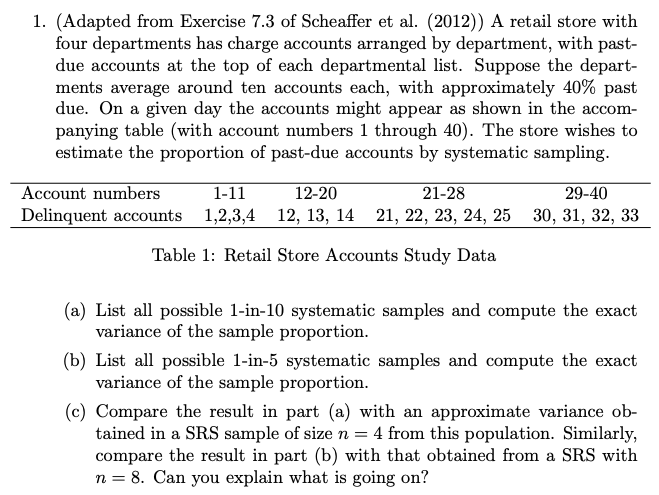
\includegraphics[width = 15cm]{img/Q1.png}
    %\caption{Section 6.1 Q8}
    %\label{fig:figure1label}
\end{figure}

~\

\subsection{(a)}
We need to fix the starting point, when start at 1: the number of deliquent accounts is 3, 
the sample proportion is $\frac{3}{4}.$ 

When start at 2: the number of deliquent accounts is 4. The sample proportion is $1.$

When start at 3: the number of deliquent accounts is 4. The sample proportion is $1.$ 

When start at 4: the number of deliquent accounts is 3. The sample proportion is $\frac{3}{4}.$ 

When start at 5: the number of deliquent accounts is 1. The sample proportion is $\frac{1}{4}.$ 

When start at 6: the number of deliquent accounts is 0. The sample proportion is $0.$ 

When start at 7: the number of deliquent accounts is 0. The sample proportion is $0.$ 

When start at 8: the number of deliquent accounts is 0. The sample proportion is $0.$ 

When start at 9: the number of deliquent accounts is 0. The sample proportion is $0.$ 

When start at 10: the number of deliquent accounts is 1. The sample proportion is $\frac{1}{4}.$ 

Therefore the exact variance of sample proportion is $0.165.$

\subsection{(b)}
When start at 1: the number of deliquent accounts is 3. The sample proportion is $0.375.$

When start at 2: the number of deliquent accounts is 4. The sample proportion is $0.5.$

When start at 3: the number of deliquent accounts is 4. The sample proportion is $0.5.$

When start at 4: the number of deliquent accounts is 3. The sample proportion is $0.375.$

When start at 5: the number of deliquent accounts is 2. The sample proportion is $0.25.$

Hence the exact variance of sample proportion is $8.75\times 10^{-3}.$

\subsection{(c)}
Using the formulae $$Var(\hat{p})=\frac{N-n}{N-1}p(1-p).$$

And we have $p=0.4, N=40,$ therefore $Var(\hat{p})=0.0554.$

For $n=8$, $Var(\hat{p})=0.0246.$

When n=4, SRS's variance is smaller and when n=8, SRS's is larger.

Because when $n=4,$ the ICC (intracluster coorelation coefficient) is tend to be larger, because
ICC represents how things are similar inside a cluster. Therefore $Var(\hat{p})$ tends to be 
underestimating.

And when $n=8$, the ICC is smaller, then $Var(\hat{p})$ tends to be overestimating.

\newpage
\section{Q2}
\begin{figure}[htp]
    \centering % 图片居中
    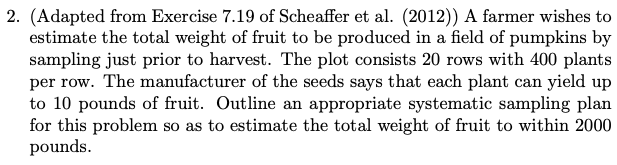
\includegraphics[width = 15cm]{img/Q2.png}
    %\caption{Section 6.1 Q8}
    %\label{fig:figure1label}
\end{figure}

~\ 

Note that we can regard every plant's condition is the same. Therefore we can apply the 
formulae from SRS: $$n=\frac{1}{\frac{1}{N} + 
\frac{d^2}{N^2v^2z_{1-\frac{\alpha}{2}}^2}(1-\frac{1}{N})}.$$

The $v$ is the "pre-sample estimate". We calculate it by $Range Rule of Thumb$, which is 
we calculate the variance by range divide by 4: $v=(10-0)/4=2.5$

And we have $N=20\times 400 = 8000,$ $d=2000,$ $z_{1-\frac{\alpha}{2}}=z_{0.975}=1.96.$

Hence we can calculate $n=366.6016.$ Therefore we take $n=367.$

And by $8000/366.6=21.8221.$ So take $k$ (the stepsize) be 21. 

To summarize, we should perform a 1-in-21 systematic sampling.


\newpage
\section{Q3}
\begin{figure}[htp]
     % 图片居中
    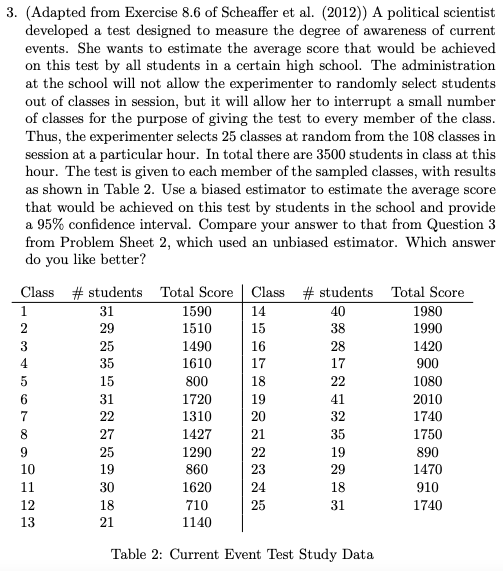
\includegraphics[width = 14cm]{img/Q3.png}
    %\caption{Section 6.1 Q8}
    %\label{fig:figure1label}
\end{figure}

~\ 

For sure we will apply the "using auxiliary data" method.

Define $X_i$ is the number of students in sampled class $i$. (E.g. 
$X_1=31$.)

Define $Y_i$ is the total score of sampled class $i$. (E.g. $Y_1=1590.$)

Hence $\bar{Y}=\frac{1}{25}\sum_{i=1}^{25}Y_i=1398.28.$ And 
$\bar{X}=\frac{1}{25}\sum_{i=1}^{25}X_i=27.12.$ 
Then $$\hat{R}=\frac{\bar{Y}}{\bar{X}}=51.5590.$$

Hence $\hat{\mu}=51.5590.$

Then using the formulae 
$\widehat{Var(\hat{\mu})}=\frac{N}{M^2}(N-n)\frac{1}{n}\hat{\sigma_r^{2}}.$ 
Where $\hat{\sigma_r^{2}}=10808.7251.$

We can gain that $\widehat{Var(\hat{\mu})}=0.3164.$

Therefore, an 95\% C.I. can be $(51.5590 \pm t_{24,0.975}\sqrt{0.3164}~)=(50.3981,52.7199).$

Recall that the result from Problem Set 2 is $(43,147 \pm 4.3081).$

I prefer the biased approach, because this has a much smaller variance.






\end{document}
